
    \begin{picture} (180.000000,128.083333)(0,0)
    \put(0.0, 0.0){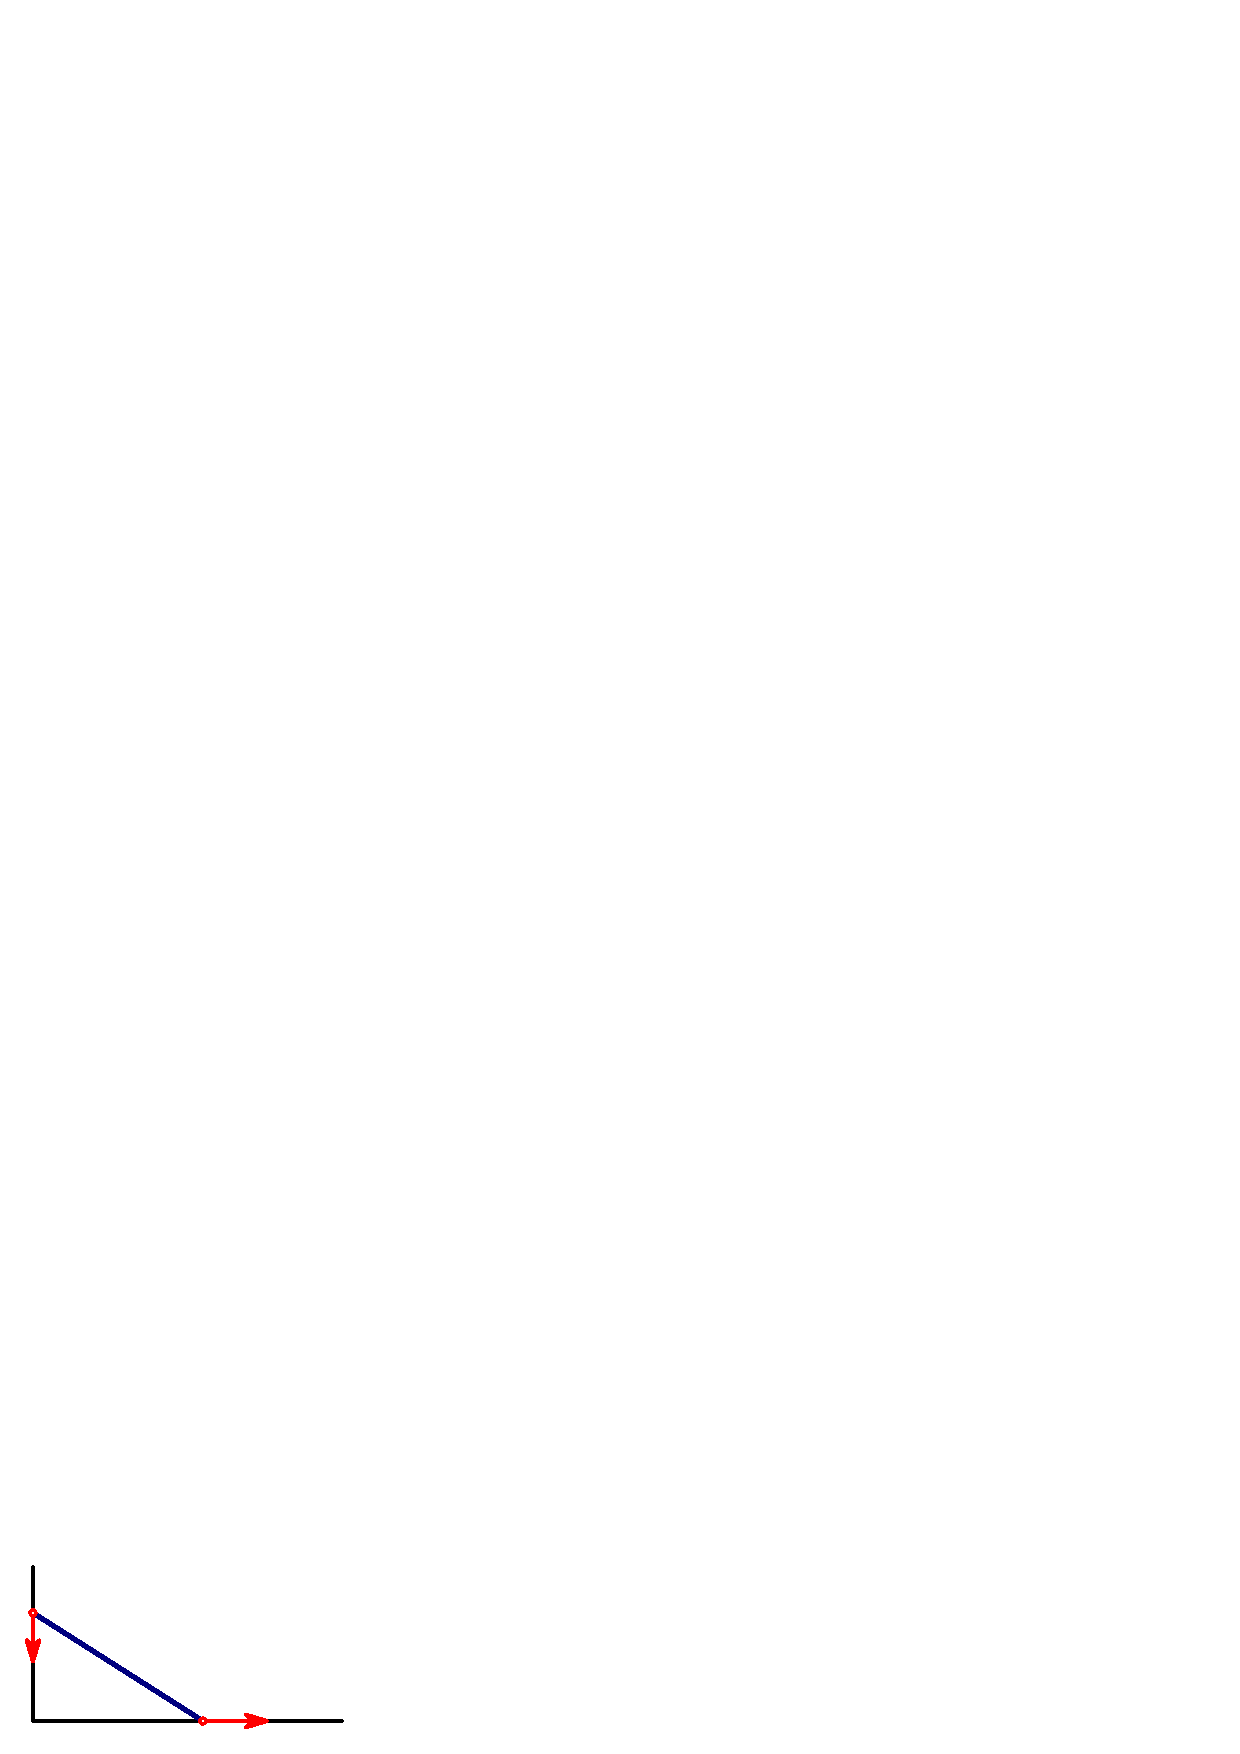
\includegraphics{04slidingPole.pdf}}
        \put( 18.83,  70.75){\sffamily\itshape $A$}
    \put( 99.42,  19.83){\sffamily\itshape $B$}
    \put( 58.62,  43.79){\sffamily\itshape \sffamily pole of length 10 ft}
    \put( -2.17,  41.79){\sffamily\itshape $a(t)$}
    \put( 52.62,   3.83){\sffamily\itshape $b(t)$}
\end{picture}
